\section{Evaluierung }
\label{sec:5}
\markboth{Evaluierung}{Evaluierung}

Beide Methoden haben ihre Vor- und Nachteile. Die realistische Darstellung von voluminösen Materialien verlangt
eine besondere Herangehensweise. Die Darstellung der Volumen lässt sich – im Gegensatz zu undurchsichtigen, festen Oberflächen – 
mit herkömmlichen Texture-Mapping-Methoden in einer VR-Umgebung nicht überzeugend darstellen.
Die Implementierung der Systeme ist aufgrund der begrenzten Zeit im Rahmen dieser Arbeit nur prototypisch mithilfe der
zur Verfügung stehenden Funktionen aus Unity implementiert, und daher nicht bestmöglich optimiert.
Einige Vor- und Nachteile, sowie das Potential für den Nutzen der jeweiligen Methoden, lassen sich dennoch aus dem Entwurf
ableiten und werden in den weiteren Abschnitten beschrieben.


\subsection{Parallax Occlusion Mapping}
\label{sec:5.1}
\begin{figure}[!h]
	\centering
	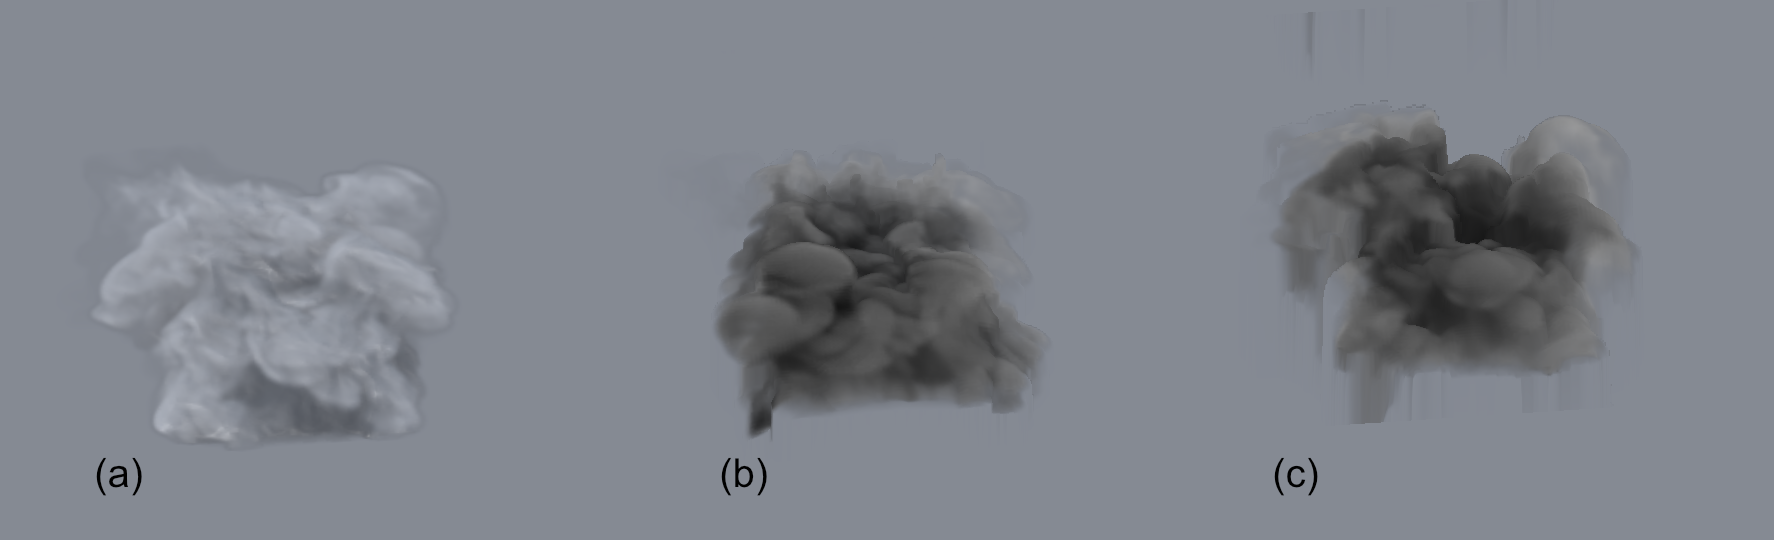
\includegraphics[width=0.89\textwidth]{Grafiken/Implementation/pom_Vergleich.png}
	\begin{footnotesize}
		\caption{Vergleich verschiedener Verfahren, aus flacherem Blickwinkel betrachtet. 
		(a) Normal Mapping, (b) 6-Punkt-beleuchtetes Parallax Occlusion Mapping, einzelner Frame der Simulation. (c) 6-Punkt-beleuchtetes Parallax Occlusion Mapping, Texture Sheet-Animation. }
		\label{fig:pomVergleich}
	\end{footnotesize}
\end{figure}

POM ist eine komplexere Variante des Normalmappings. Dementsprechend ist auch diese Technik eher für feste Oberflächen und weniger
für den Einsatz bei der Simulation von Volumen gedacht. Um aber die Effizienz der Billboard-basierten Partikelsysteme
nutzen zu können, ist das Parallax Occlusion Mapping aber eine interessante Möglichkeit, die es wert ist, getestet zu werden. 
Vorallem für die Anwendung bei dichtem, schwarzen Rauch mit geringer Transparenz, bei dem die äußere Schicht bei Betrachtung aus weiterer 
Entfernung beinahe wie eine solide Oberfläche erscheinen könnte. 

In \textbf{\autoref{fig:pomVergleich}} ist ein Vergleich der Variante von POM mit einem einzelnen Sprite, sowie einer Animation, basierend auf einem Texture Sheet, zu sehen. 
Auf der linken Seite befindet sich ein Frame der Simulation ohne Parallax Offsetting, lediglich mit einer Normal Map. Dieser Vergleich macht den Vorteil der 6-Punkt-Beleuchtung und 
des Parallax Occlusion Mappings gegenüber herkömmlichen Mappingverfahren deutlich. 
Bei der Betrachtung in VR entsteht ein realistischerer Eindruck von Tiefe, da sich blickwinkelabhängig verschiedene Teile der Textur gegenseitig verdecken. Gerade wenn sich beim Betrachten
um die Textur herum bewegt wird, verstärkt sich dieser Effekt.  
Dies bestätigt die Vermutung, dass sich POM für VR deutlich mehr eignet als herkömmliches Normal Mapping. Jedoch gilt dies nur für das Standbild des Rauches.
Auf der rechten Seite sieht man deutlich, wie sich die benachbarten Frames bei der Animation des Rauches mit in den sichtbaren Bereich hineingezerrt werden.
Ein weiteres Problem der Texture Sheet-basierten Animation sind die Randflächen des Rauches. Dadurch, dass die Höhe an der Umrandung des Rauches in der Textur unmittelbar abfällt,
werden einige Pixel, die an einer solchen Schnittkante liegen, stark verzogen. Selbst bei geringem Pixeloffset, bei dem sich der Parallax-Effekt noch kaum bemerkbar macht. 
Auch dies ist in \textbf{\autoref{fig:pomVergleich}} erkennbar. Da sich der Rauch mit jedem Frame verändert, springen
die Artefakte entlang der Randflächen. Der Effekt tritt stärker auf, wenn zunächst die Animation durchlaufen und daraufhin das Pixeloffset berechnet wird. Die Artefakte lassen sich 
reduzieren, indem die Rehenfolge der UV-Manipulationen umgekehrt wird. Die Implementierung des POM Nodes von Unity verhindert damit jedoch die Animation der Heightmap, was 
die Texture Sheet-Animation – in Kombination mit Parallax Occlusion Mapping – in der Art und Weise, wie sie hier implementiert ist, unbrauchbar macht. 

In Anbetracht der Performance läuft die Anwendung auf dem Testsystem in einer VR-Umgebung, stabil mit 90FPS. Trotz der erhöhten Komplexität des Algorithmus gegenüber klassischeren 
Mappingverfahren hält sich der Rechenaufwand in Grenzen. Hier gibt es also keine Bedenken hinsichtlich der Shaderlaufzeit. Auch die aufwändige Berechnung der Fluidsimulationen wird hier im Voraus erledigt. 
Somit ist es möglich, realistisch aussehende Partikelsysteme unter geringem Rechenaufwand in der Echtzeitanwendung zu erzeugen. Ein weiterer Vorteil, der sich aus der Natur des schwarzen 
Rauches bei Bränden ergibt, ist die Tatsache, dass die genaue Berechnung von Selbstschattierungen hierbei nicht so essentiell ist wie bei weißem Rauch. Dies ist zwar nicht direkt ein Vorteil von POM, 
gleicht aber einen Nachteil aus, den es in der Anwendung in einem Partikelsystem gibt: Die Texturen auf den Billboards sind in der Lage, sich individuell selbst zu schattieren. 
Eine gegenseitige Schattierung ist jedoch ohne weiteres nicht möglich (vgl. \textbf{\autoref{fig:pomShadows}}). 
In Bezug auf Schattierung im Allgemeinen gibt es das Problem, dass Billboard-basierte Partikelsysteme eigentlich nur flache Sprites sind und deshalb nicht in der 
Lage sind, realistische Schatten auf die Umgebung werfen zu können. 



\begin{figure}[h!]
	\centering
	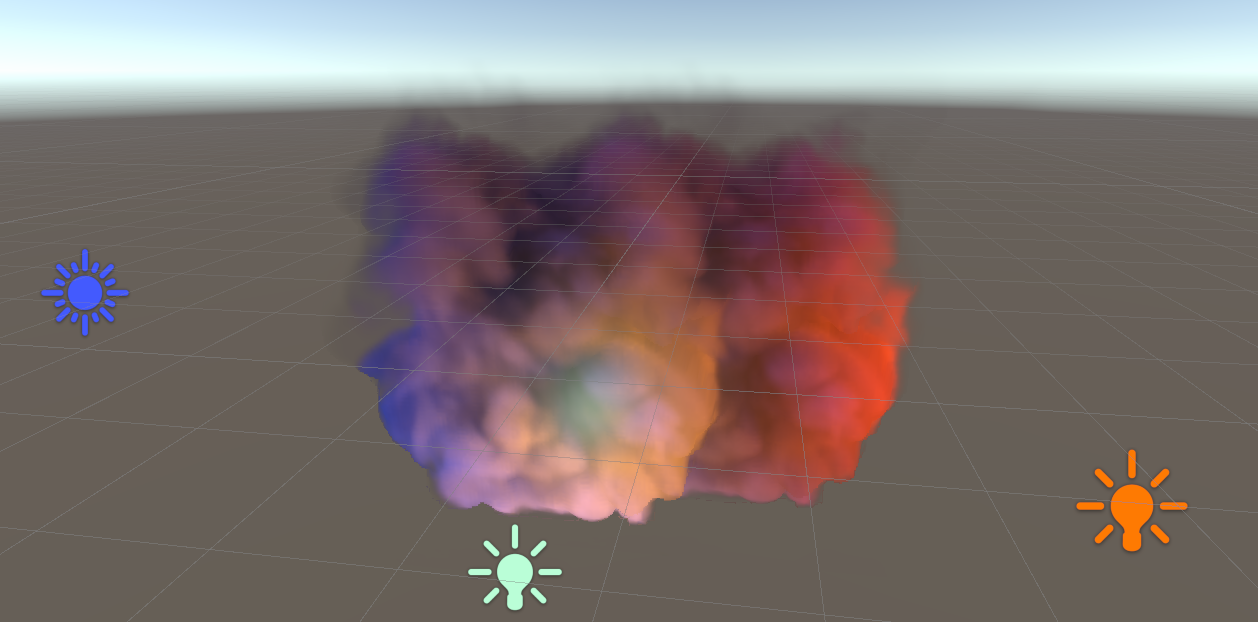
\includegraphics[width=0.89\textwidth]{Grafiken/Evaluation/pomShadows.png}
	\begin{footnotesize}
		\caption{Kein gegenseitiger Schattenwurf bei POM-basierten Billboards. }
		\label{fig:pomShadows}
	\end{footnotesize}
\end{figure}

\begin{figure}[h!]
	\centering
	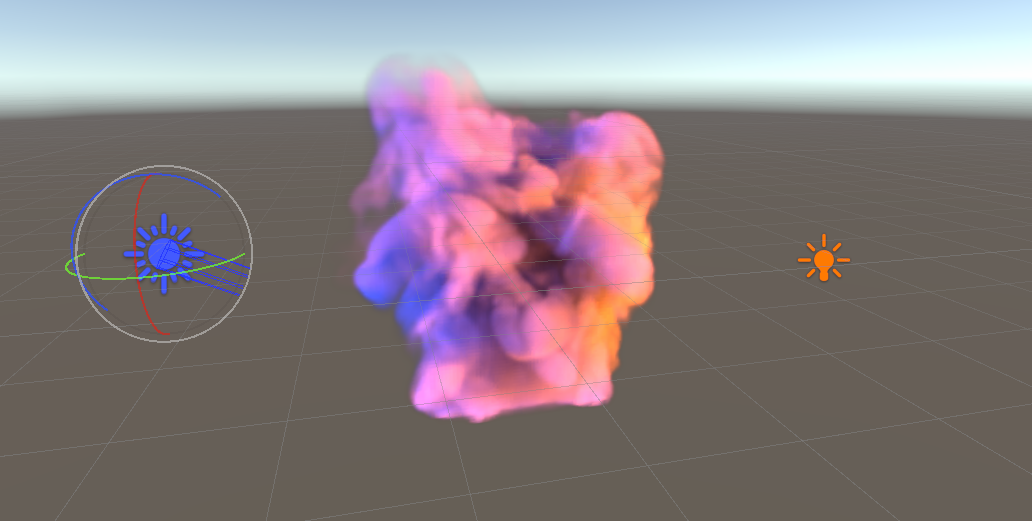
\includegraphics[width=0.89\textwidth]{Grafiken/Implementation/litSmoke.png}
	\begin{footnotesize}
		\caption{Dynamische Beleuchtung des Rauchs}
		\label{fig:dynamicLightingSmoke}
	\end{footnotesize}
\end{figure}


Ein weiterer Vorteil, der sich aus dieser Methode ergibt, sind die Texture Sheets. In eine einzige Textur lassen sich 4 verschiedene Informationen in die
RGBA-Kanäle speichern. Neben den verschiedenen Lightmaps aus 6 Richtungen können beispielsweise noch Farbinformationen oder Emission- und Heatmaps gespeichert werden.
Mit weiteren Infos wie einer Heatmap lässt sich ein Übergang, bzw. eine Mischung von Feuer und Rauch erzeugen. Dies ist ein Phänomen, welches sich bei größeren Bränden
oder Explosionen beobachten lässt (vgl. \textbf{\autoref{fig:explosion}}).
Die Anzahl der Lightmaps lässt sich auch reduzieren, indem die Lichtrichtungen von vorne und von hinten im Shader approximiert werden.
Es gibt viele Möglichkeiten, die Flexibilität von Texturen ausnutzen zu können und dabei die Menge an benötigten Daten und Berechnungen gering zu halten,
sodass der flüssige Einsatz in VR gegeben bleibt. Weiterhin lassen sich auf Kosten weiterer Texture Sheets
verschiedene Simulationen erstellen, sodass größere Varianz in das Aussehen des Partikelsystems eingebracht werden kann.
Durch die unendliche Wiederholbarkeit kann die Animation ab einem zufällig gewählten Frame starten, wodurch schon mit einer einzigen Animation mit genug Frames
kaum auffällt, dass das ganze System auf lediglich einer einzigen Sequenz aufbaut.


Neben den ganzen Vorteilen, die diese Variante mit sich bringt, gibt es auch negative Punkte. Bei zu geringer Auflösung sehen die Renderings schnell
verpixelt aus, je näher diese betrachtet werden. Dies ist ein großer Nachteil der Texture Sheets. Wird die Auflösung jedes Frames verdoppelt, also in diesem
Fall von 256x256 Pixel auf 512x512 Pixel, so erhöht sich die Auflösung der gesamten Textur um den Faktor vier für jeden der RGBA-Kanäle. Selbst dann sind
die einzelnen Frames noch relativ gering aufgelöst und nicht für die Betrachtung aus der Nähe gedacht. Je detaillierter die Simulation, auf denen die Texture Sheets basieren,
desto höher sollte die Auflösung sein, um auch alle diese Details abbilden zu können.
Die visuellen Artefakte, wie beispielsweise das Einschneiden der benachbarten Frames aus dem Texture Sheet aus einem flachen Betrachtungswinkel (vgl. \textbf{\autoref{fig:smokeBleeding}}),
schränken die Einsatzmöglichkeiten für die Anwendung in VR stark ein. Die Verzerrung am Rand, welche durch eine starke Kante in der Heightmap hervorgerufen wird, macht das
Parallax Occlusion Mapping ebenfalls für die Darstellung von voluminösen Medien ungeeignet. Zudem ist der Parallax Effekt bei Billboards, die immer von vorne betrachtet werden, so schwach, 
dass sich der Aufwand der Berechnungen nicht wirklich lohnt. 
Bei der Darstellung des Feuers kommt der Faktor hinzu, dass Billboards nicht als Lichtquelle fungieren, was dem Realismus der Simulation schadet.

Abschließend lässt sich zu dem Rendering von Feuer und Rauch auf Basis von Parallax Occlusion Mapping sagen, dass sich diese Variante, so wie sie für diese Arbet
implementiert ist, nicht immer eignet. Die visuellen Artefakte erzeugen Störungen der Immersion. Jedoch wird das Parallax Offset in der Stereoansicht korrekt dargestellt,
wodurch dieser Ansatz vielversprechend bleibt. Es ist wahrscheinlich, dass es für die genannten Probleme elegante Lösungen gibt, die in Zukunft an anderer Stelle 
betrachtet werden könnten.


\begin{figure}[h!]
	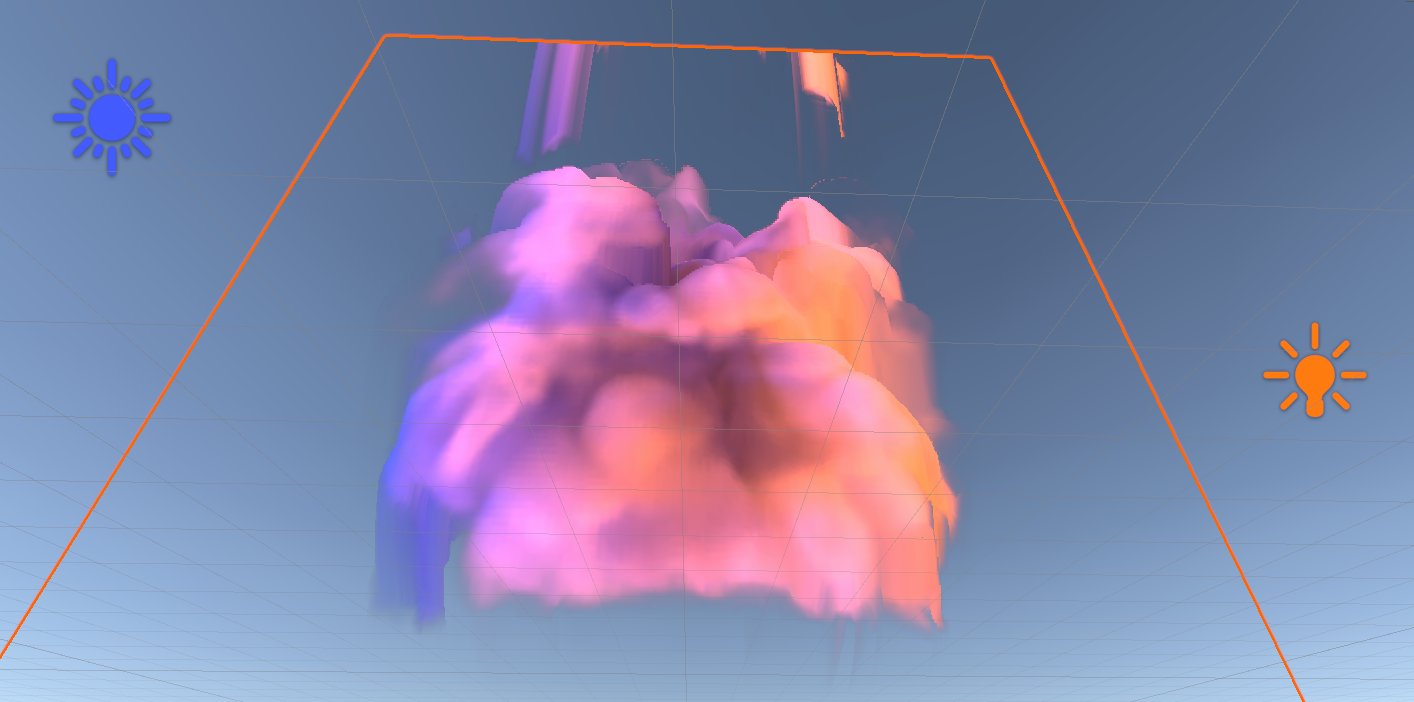
\includegraphics[width=0.89\textwidth]{Grafiken/Evaluation/Smoke_artefacts.png}
	\centering
	\begin{footnotesize}
		\caption{Verzerrungsartefakte bei der Anwendung von Parallax Occlusion Mapping mit zu starkem Offset. Die benachbarten Frames des Texture Sheets
			werden ebenfalls mit verzerrt, wodurch Fragmente davon, bei flachem Betrachtungswinkel, mit in das Billboard einlaufen.}
		\label{fig:smokeBleeding}
	\end{footnotesize}
\end{figure}



\subsection{Ray Marching}
\label{sec:5.2}

Aufgrund der massiven Einschränkungen in der Qualität des Exports aus Houdini wurde (für die bessere Betrachtung in VR) ein Set Volume Slices aus dem 
Github-Repository von Dylan Meville verwendet\footnote{\url{https://github.com/DMeville/DMVolumeRendering/blob/main/DMVolumeRendering/Assets/VolumeRubberCube.exr}, abgerufen am 28.07.2022}.
Zudem konnte im zeitlichen Rahmen dieser Arbeit, aufgrund vieler Probleme mit der Entwicklung der Shader, leider nur eine simple Implementierung des Volume Ray Marching Ansatzes für das Rendering 
von 3D-Texturen entwickelt werden (vgl. \textbf{\autoref{fig:rubber}}). Dieser reagiert nicht auf das Licht der Umgebung, hier wird lediglich die Dichte des Volumens abgetastet. 
Dies kann jedoch in VR betrachtet werden und zeigt bereits Vorteile auf.  
Daher werden im Folgenden nun die theoretischen Vor- und Nachteile des Volume Ray Marchings erläutert.

\begin{figure}[h!]
	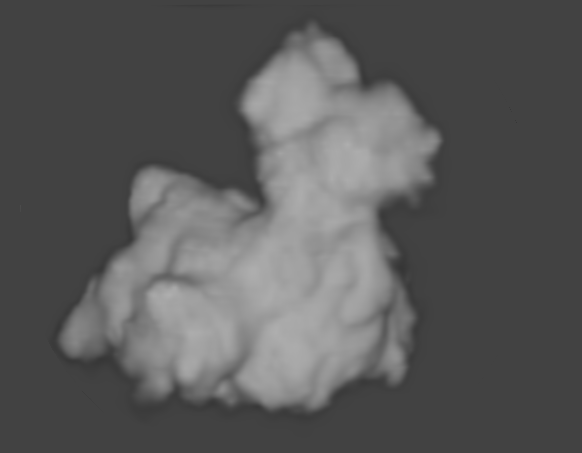
\includegraphics[width=0.49\textwidth]{Grafiken/Evaluation/raymarch/rubberDuck.png}
	\centering
	\begin{footnotesize}
		\caption{Volumenrendering der Dichte einer 3D-Textur. Quelle: \parencite{Shaderbits:Volume}}
		\label{fig:rubber}
	\end{footnotesize}
\end{figure}

Der Ansatz des Volume Renderings auf Basis von Ray Marching könnte sich besonders gut für die Darstellung von Effekten wie Feuer und Rauch eignen. 
Die Tatsache, dass das Volumen nicht nur vorgetäuscht, sondern tatsächlich dargestellt werden kann, macht das Rendering sehr realistisch. 
Während die Volumen durchlaufen werden, wird schrittweise die Farbe, die Dichte, sowie die Lichtintensität in den einzelnen Voxels berechnet und zusammen geführt. 
Daraus sollte sich ein qualitativ hochwertiges Shading der Rauchwolken ergeben. Gerade für die Betrachtung in VR ist dieser Ansatz besonders vielversprechend. 
Die Volumen sehen, aus allen Richtungen betrachtet, realistisch aus und können auf theoretisch auf dynamische Beleuchtung reagieren (vgl. \textbf{\autoref{fig:rayM}}). 
Zudem können Volumen das durchlaufende Licht nicht nur absorbieren und reflektieren, sondern auch selbst emittieren. Durch diese Eigenschaft kann das
emittierte Licht die Umgebnung nicht nur schattieren, sondern auch beleuchten. 

\begin{figure}[h!]
	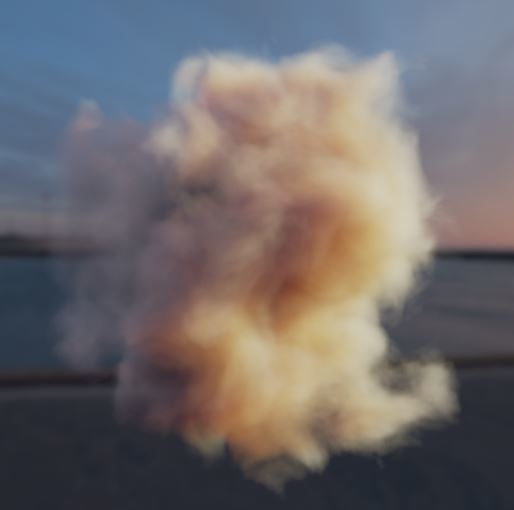
\includegraphics[width=0.79\textwidth]{Grafiken/Evaluation/raymarch/Smokeball.JPG}
	\centering
	\begin{footnotesize}
		\caption{3D-Volumen mittels Volume Ray Marching gerendert. Bei dem Shading des Volumens wird das durchfallende Licht mit einbezogen. Quelle: \parencite{Shaderbits:Volume}}
		\label{fig:rayM}
	\end{footnotesize}
\end{figure}


Verfolgt man die Lichtstrahlen durch die Volumen weiter, so könnten mit geringem Mehraufwand auch realistische Schattierungen der Umgebung berechnet werden. 
Wurde ein Volumen, bzw. eine Szene, mittels Ray Marching abgelaufen, so können, ebenfalls mit geringem Aufwand, weitere Effekte, wie 
Ambient Occlusion oder Reflektionen berechnet werden. All dies sind Faktoren, die zu einem realistischeren Rendering beitragen.

Ebenso wie Parallax Occlusion Mapping, werden die Berechnungen hier für jeden Pixel vorgenommen.
Das heißt, dass aufgrund der Natur des Ray Marching Algorithmus, ohne Probleme für jedes Auge eine korrekte Darstellung geliefert werden kann. 
Dabei muss jedoch gerade in VR-Umgebungen die Performance beobachtet werden. 
In der Testszene lief die Betrachtung des ray marched Rauches mit einer stabilen Frame Rate oberhalb der 90FPS-Grenze. In größeren, komplexeren Umgebungen 
macht sich gelegentlich ein Einbruch der Frame Rate bemerkbar. 
Mit steigender Komplexität der Berechnungen, beispielsweise durch die zusätzlichen Effekte oder komplexere Szenen, könnte die Performance weiter leiden. 
Dennoch eignet sich theoretisch auch diese Methode für die Anwendung in VR. 

Ein Nachteil der vorgeschlagenen Implementierung des Volume Ray Marching liegt bei den notwendigen 3D-Texturen. 
Die Texturen auf Basis der Fluidsimulationen sind statisch und lassen sich nicht realistisch animieren. Lediglich die Texturen, basierend auf dem
generierten Rauschen, können animiert werden, haben aber den Nachteil, dass diese weniger realistisch aussehen. Diese Texturen würden sich eher anbieten,
um weit entfernte Wolken oder Nebel zu erzeugen. Der dichte, schwarze Rauch, der bei einem großen Feuer erzeugt wird, lässt sich nicht überzeugend 
durch solche Texturen darstellen. 

Letztendlich ist der Volume Ray Marching-Ansatz jedoch auch sehr vielversprechend und kann in einer Simulation in VR gut verwendet werden. 
Die Methode bietet einige Möglichkeiten der Optimierung und erzeugt ein plausibles Bild für den Betrachter. 
Für die Anwendung in einem Partikelsystem für Feuer und Rauch muss jedoch noch eine Möglichkeit gefunden werden, den Rauch zu animieren oder 
realitätsnah geformt werden zu können. 